% $Header$

\documentclass{beamer}

% Copyright (c)  2021  HiKlas Ltd.
% Permission is granted to copy, distribute and/or modify this document
% under the terms of the GNU Free Documentation License, Version 1.3
% or any later version published by the Free Software Foundation;
% with no Invariant Sections, no Front-Cover Texts, and no Back-Cover Texts.
% A copy of the license is included in the section entitled "GNU
% Free Documentation License".
%
% Based on the Beamer generic-ornate-15min-45min.en.tex template by
% Till Tantau <tantau@users.sourceforge.net>



\mode<presentation>
{
  \usetheme{CambridgeUS}
}

\usepackage[english]{babel}
\usepackage[latin1]{inputenc}
\usepackage[T1]{fontenc}
% Or whatever. Note that the encoding and the font should match. If T1
% does not look nice, try deleting the line with the fontenc.

% These packages are used for drawing circuits
\usepackage{tikz}
\usepackage[siunitx,european,americanresistors]{circuitikz}

% Packages for mathematical notation
\usepackage{amsmath}

% Trying to split long URLs across lines
% From this post suggesting breakurl: https://stackoverflow.com/questions/2640111/url-latex-linebreak
% The breakurl package: https://ctan.org/pkg/breakurl?lang=en
% Example of options: https://tex.stackexchange.com/questions/298851/linebreak-in-long-url-breakurl-wont-break-it
\usepackage{hyperref}
\usepackage[hyphenbreaks]{breakurl}

% Information about the presentation 
\title{Introduction to Machine Code}
\subtitle{002 Processors}
\author{Fiona Bianchi}
\institute{HiKlas Ltd}
\date{August 2021}
\subject{Talks}
\pgfdeclareimage[height=0.5cm]{company-logo}{../assets/HiklasLogo.eps}
\logo{\pgfuseimage{company-logo}}

% Table of contents for each Subsection
\AtBeginSubsection[]
{
  \begin{frame}<beamer>{Outline}
    \tableofcontents[currentsection,currentsubsection]
  \end{frame}
}

% TODO: Nope, I don't think I want this put leaving it in just in case
% TODO: to remove when absolutely sure
% If you wish to uncover everything in a step-wise fashion, uncomment
% the following command: 
%\beamerdefaultoverlayspecification{<+->}

% Show the notes
\ifdefined\isnotes
\setbeameroption{show only notes}
\fi

% Show notes and slides
\ifdefined\ishandout
\setbeameroption{show notes}
\fi


\begin{document}

\begin{frame}
  \titlepage
\end{frame}

\begin{frame}{Outline}
  \tableofcontents
  % TODO: What is "pausesections" for?
  % You might wish to add the option [pausesections]
\end{frame}

\section{What do processors look like?}

\subsection[Precursors]{Very old}

\begin{frame}{Babbage Difference Engine}
  \begin{columns}
    \column{0.5\textwidth}

    \begin{itemize}
    \item
      Designed by Charles Babbage \cite{BabbageBio}
      \note[item]{Implementation of No.0 and partial No.1}
      \note[item]{Designed No.2 Difference Engine}
      \note[item]{No.0 was completed in 1822}
    \item
      Completely mechanical calculating engine 
    \item
      Superseded in design by analytical engine \cite{AnalyticalEngine}
      \note[item]{Only designed never implemented in Babbage's lifetime}
      \note[item]{General purpose computer design with processor, memory}
      \note[item]{ALU - Arithmetic and Logic unit: tests, branches, loops}
      
    \end{itemize}

    \column{0.50\textwidth}
    \begin{center}
      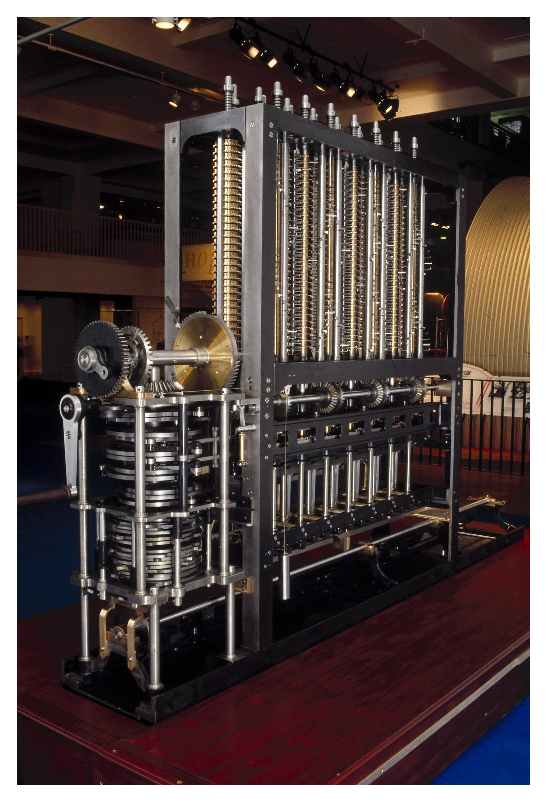
\includegraphics[scale=0.4]{../assets/Difference_Engine_London.eps}
      \cite{BabbageEngine} Difference Engine No.2
    \end{center}

  \end{columns}
\end{frame}


\subsection[Firsts]{Old}

\begin{frame}{Colossus}
  \begin{columns}
    \column{0.5\textwidth}
    
    \begin{itemize}
    \item
      Something
    \end{itemize}
    
    \column{0.50\textwidth}
    \begin{center}
      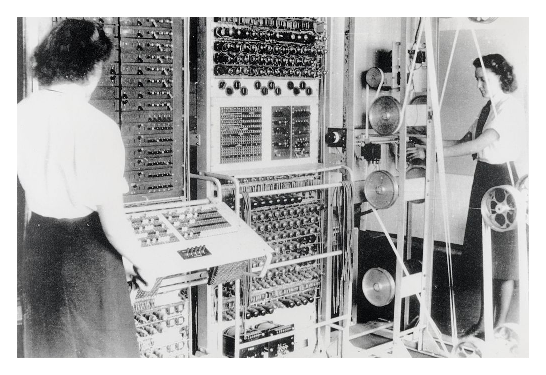
\includegraphics[scale=0.4]{../assets/ColossusOperation.eps}
      \cite{Colossus1943} Colossus Operating in 1943
    \end{center}
    
  \end{columns}
\end{frame}

\begin{frame}{Colossus Rebuild}
  \begin{columns}
    \column{0.75\textwidth}
    
    \begin{itemize}
    \item
      Something
      
    \end{itemize}
    
    \column{0.25\textwidth}
    \begin{center}
      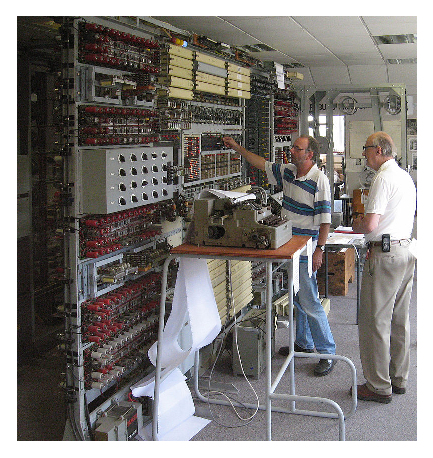
\includegraphics[scale=0.4]{../assets/ColossusRebuild_11.eps}
      \cite{ColossusRebuild} Colossus Rebuild
    \end{center}
    
  \end{columns}
\end{frame}


\subsection[Modern]{Current}

\begin{frame}{A frame}
  \begin{itemize}
  \item
    One item
  \item
    Two item
  \end{itemize}
\end{frame}



\section{What do processors do?}

\subsection[Maths]{Simple maths}

\begin{frame}{Whole Numbers}
  \begin{itemize}
  \item
    Addition, Subtraction, Multiplication, Division
  \item
    Add/Subtract easy in hardware
  \item
    Multiply/divide more complicated
  \item
    Fixed sized numbers, 8bit, 16bit, 32bit, 64bit
  \end{itemize}
\end{frame}

\begin{frame}{Logical Operations}
  \begin{itemize}
  \item
    Again fixed size numbers
  \item
    Operations on binary bits
  \item
    AND, OR, XOR, NOT
  \item
    Used for transforming or manipulating data (bitmasks for example)
  \end{itemize}
\end{frame}

\begin{frame}{Comparisons and Tests}
  \begin{itemize}
  \item
    Greater than, less than, equal to zero
  \item
    Used as conditions on branches, e.g. branch if not zero
  \item
    Uses basic maths operations, e.g. subtract
  \item
    Maths operations can trigger carry flag
  \end{itemize}
\end{frame}


\subsection[Memory]{Remembering Data}

\begin{frame}{Types of Memory}
  \begin{itemize}
  \item
    Registers: inside the processor
  \item
    Cache: also often on the same die as the CPU
  \item
    RAM: Random Access Memory - read/write
    \begin{itemize}
    \item
      Static RAM (SRAM)
    \item
      Dynamic RAM (DRAM)
    \end{itemize}
  \item
    ROM: Read Only memory
    \begin{itemize}
    \item
      EPROM: Erasable Programmable Read Only Memory
    \item
      EEPROM: Electrically Eraseable
    \end{itemize}
  \end{itemize}
\end{frame}

\subsection[IO]{Input/Output}

\begin{frame}{A frame}
  \begin{itemize}
  \item
    One item
  \item
    Two item
  \end{itemize}
\end{frame}

\section{Programming Processors}

\subsection[Older]{Beginnings}

\begin{frame}{A frame}
  \begin{itemize}
  \item
    One item
  \item
    Two item
  \end{itemize}
\end{frame}

\subsection[Assembly]{Assembly Language}

\begin{frame}{A frame}
  \begin{itemize}
  \item
    One item
  \item
    Two item
  \end{itemize}
\end{frame}


\subsection[Compilers]{Compilers}

\begin{frame}{A frame}
  \begin{itemize}
  \item
    One item
  \item
    Two item
  \end{itemize}
\end{frame}





\section{Summary}

\begin{frame}{Summary}

  % Keep the summary *very short*.
  \begin{itemize}
  \item
    Item one
  \item
    Item two
  \end{itemize}
  
  % The following outlook is optional.
  \vskip0pt plus.5fill
  \begin{itemize}
  \item
    Outlook
    \begin{itemize}
    \item
      Something you haven't solved.
    \item
      Something else you haven't solved.
    \end{itemize}
  \end{itemize}
\end{frame}


\section{Bibliogrphy}

\begin{frame}{Bibliography 1}
  \frametitle{References}
  
  \begin{thebibliography}{Babbage Difference Engine}
  \bibitem[Babbage Difference Engine]{BabbageEngine}
    Science Museum London, Difference Engine No.2
    \newblock {\url{https://collection.sciencemuseumgroup.org.uk/objects/co526657/difference-engine-no-2-designed-by-charles-babbage-built-by-science-museum-difference-engine}}

  \bibitem[Babbage Biography]{BabbageBio} 
    Charles Babbage Biography with references
    \newblock {\url{https://mathshistory.st-andrews.ac.uk/Biographies/Babbage/}}

  \bibitem[Analytical Engine]{AnalyticalEngine}
    Babbage Analytical Engine
    \newblock {\url{https://en.wikipedia.org/wiki/Analytical_Engine}}

  \bibitem[Colossus]{Colossus}
    The rebuild colossus at \cite{TNMOC} TNMOC
    \newblock {\url{https://www.tnmoc.org/colossus}}

  \end{thebibliography}
\end{frame}

\begin{frame}{Bibliography 2}
  \frametitle{References}
  
  \begin{thebibliography}{ColossusRebuild}
  \bibitem[TNMOC]{TNMOC}
    The National Museum Of Computing
    \newblock {\url{https://www.tnmoc.org/}}
    
  \bibitem[Bletchley Park]{Bletchley}
    Bletchley Park
    \newblock {\url{https://bletchleypark.org.uk}}
    
  \bibitem[Colossus Operation]{Colossus1943}
    Colossus being operated by Dorothy Du Boisson (left) and Elsie Booker (right)
    \newblock {\url{https://en.wikipedia.org/wiki/Colossus_computer\#/media/File:Colossus.jpg}}

  \bibitem[Colossus Rebuild]{ColossusRebuild}
    Rebuild of Colossus supervised by Tony Sale (Right)
    \newblock {\url{https://en.wikipedia.org/wiki/Colossus_computer\#/media/File:ColossusRebuild_11.jpg}}
  \end{thebibliography}
\end{frame}


\end{document}
